\documentclass{article}%
\usepackage[T1]{fontenc}%
\usepackage[utf8]{inputenc}%
\usepackage{lmodern}%
\usepackage{textcomp}%
\usepackage{lastpage}%
\usepackage{geometry}%
\usepackage{float}%
\usepackage{biblatex}%
\usepackage{amsmath}%
\usepackage{animate}%
\usepackage{subcaption}%
\usepackage{hyperref}%
\addbibresource{citations.bib}%
\geometry{tmargin=0.5cm,lmargin=0.5cm,rmargin=0.5cm}%
\usepackage{graphicx}%
\setlength{\parskip}{0.2em}%
%
\title{Solving and simulating the one dimensional energy balance model}%
\date{}
%
\begin{document}%
\normalsize%
\maketitle%

%
\section{Introduction}%
\label{sec:Introduction}%
The climate is a complex system made up of many moving components that interact with eachother.
It has been the dream of many scientists to make predictions about the climate, a dream which became more prevalent with onset of the 'computer age'. Notably Von Neumann the "intellectual father" of this deterministic dream, built his first computer with the
intention of "controlling the weather". \cite{Gleick}. In fact it was the ENIAC, one of the early computers that Von Neumann worked on, which had some success in numerically solving a model of the climate. \cite{Charney}
In this report, I will focus on a simple one dimensional energy balance model, derived by Budyko \cite{Budyko} and Sellers \cite{Sellers} and solve this numerically using python.
%
\section{The one dimensional energy balance model}

\subsection{The Budyko-Sellers model}
The Budyko-Sellers model describes the energy balance of the earth as
\begin{equation}
  C \frac{\partial T}{\partial t} = \frac{S(\theta)}{4} (1 - \alpha(\theta)) - \tau(\theta)\sigma T^{4} + \frac{K(\theta)}{\cos(\theta)} (\cos(\theta)\frac{\partial T}{\partial \theta})
\end{equation}

Here C is the specific heat capacity of the earth. The first term on the right hand side is the solar insolation absorbed by the earth taking into account the fraction of radiation reflected, known as the albedo, $ \alpha$. The second term is the output radiation of the earth modelled by the Stefan-Boltzman law, taking into account the fraction of radiation absorbed in the atmosphere, $\tau$. 
The third term is the heat flow at latitude $ \theta $ governed by Fourier's law. 

\subsection{Derivation of the finite difference equation for the Budyko-Sellers Model}%
\label{sec:Derivation of the finite difference equation for the Budyko-Sellers Model}%

Beginning with the Budkyo-Sellers model which is a one-dimensional energy balance model:

Let $ x = \sin(\theta)$, substituting x for $\theta$ in equation (1) gives:

\begin{equation}
  \frac{C}{K} \frac{\partial T}{\partial t} + 2x \frac{\partial T}{\partial x} + (x^2 + 1)\frac{\partial^2 T}{\partial x^2} = \frac{S_{0}}{4K}(1 - \alpha) - \frac{\tau \sigma T^4}{K} 
\end{equation}
For simplification let, 
$$
  C_{1}(x) = \frac{C}{K},
$$
$$
  C_{2}(x) = \frac{S_{0}}{4K}(1 - \alpha),
$$
$$
  C_{3}(x) = \frac{\tau \sigma}{K}  
$$

We can now introduce our finite difference equations. 

\begin{equation}
  \frac{\partial T}{\partial t} = \frac{T_{m, n +1} - T_{m, n}}{\Delta t}
\end{equation}

\begin{equation}
  \frac{\partial T}{\partial x} = \frac{1}{2}( \frac{T_{m+1, n} - T_{m,n}}{\Delta x} + \frac{T_{m, n} - T_{m-1, n}}{\Delta x})
\end{equation}

\begin{equation}
  \frac{\partial^2 T}{\partial x^2} = \frac{T_{m+1, n} - 2T_{m,n} + T_{m-1, n}}{\Delta x^2}
\end{equation}

Substituting (3), (4) and (5) into (2):

$$
  \frac{C_{1}(x)}{\Delta t}  (T_{m, n +1} - T_{m, n}) + \frac{x_{n}}{\Delta x}(T_{m+1, n} - T_{m-1, n}) + \frac{x_{n}^{2} - 1}{\Delta x^2}(T_{m+1, n} - 2T_{m,n} + T_{m-1, n}) = C_{2}(x) - C_{3}(x) T^4
$$

Rearranging for $T_{m,n+1}$,

\begin{equation}
  T_{m, n +1} =  (1 + \frac{2\beta}{c})T_{m, n} - \frac{1}{c}({\beta + \gamma})T_{m+1, n} + \frac{1}{c}(\gamma - \beta)T_{m-1, n} + \frac{1}{c}C_{2}(x) - \frac{1}{c}C_{3}(x) T^4
\end{equation}

Where:
 $$\gamma = \frac{x_{n}}{\Delta x}$$ $$\beta = \frac{x_{n}^2 - 1}{\Delta x^2}$$ $$c = \frac{C_{1}(x)}{\Delta t}$$
\subsection{Von Neuman Boundary condition}
From the Von Neuman boundary condition, we can state that there is no heat flowing at each pole. 

\begin{equation}
  \frac{\partial T}{\partial x} \Bigr|_{\substack{m = \pm 1}} = 0
\end{equation}

In order to find the temperature given at both poles a Taylor expansion is used for the subsequent values for the cases x =$\pm$ 1:

$$T_{m+1} = T_{m} + \frac{\partial T}{\partial x} \Bigr|_{\substack{m = \pm 1}} \Delta x + \frac{1}{2} \frac{\partial^2 T}{\partial x^2} \Bigr|_{\substack{m = \pm 1}}(\Delta x)^2 + ...$$
$$T_{m+2} = T_{m} + \frac{\partial T}{\partial x} \Bigr|_{\substack{m = \pm 1}} 2\Delta x + \frac{1}{2} \frac{\partial^2 T}{\partial x^2} \Bigr|_{\substack{m = \pm 1}}(2\Delta x)^2 + ...$$

Eliminating the second order of the expansion leaves:

$$ 4T_{m+1} - T_{m+2} = 3T_{m} + 2(\Delta x)\frac{\partial T}{\partial x} \Bigr|_{\substack{m = \pm 1}} $$

However, from equation (7) we can say:

\begin{equation}
  T_{m} = \frac{4T_{m+1} - T_{m+2}}{3}
\end{equation}

(At the south pole we use the two preceeding values of m-1 and m-2).


\section{Implementation of the finite difference model}
\subsection{Methodology}
I used python to generate the solutions to the finite difference model derived from above. The code can be accessed here [\url{https://github.com/Birr0/physics_labs/tree/main/climate_modelling}].

\subsection{Initial results under basic parameter assumptions}
I first ran the simulation for the following parameters;
$\tau = 0.6$ and $K = 0.5$ for 50 points of latitude over 5000 timesteps across 30 years.
The temperature for each latitidue evolved over time eventually settling to an equlibrium value.
Figure 1 (a) shows the evolution of temperature for a number of significant latitudinal positions including the poles and the equator. 
The middle line represents the global average temperature evolution over the time series.

\begin{figure}[H]%
  \centering%
  \begin{subfigure}{0.4\textwidth}
    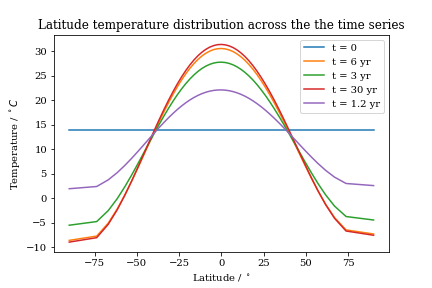
\includegraphics[width=225px]{multi-time-temp-distribution.png}%
    \caption{Latitidunal- temperature for various time series }%
  \end{subfigure}
  \begin{subfigure}{0.4\textwidth}
    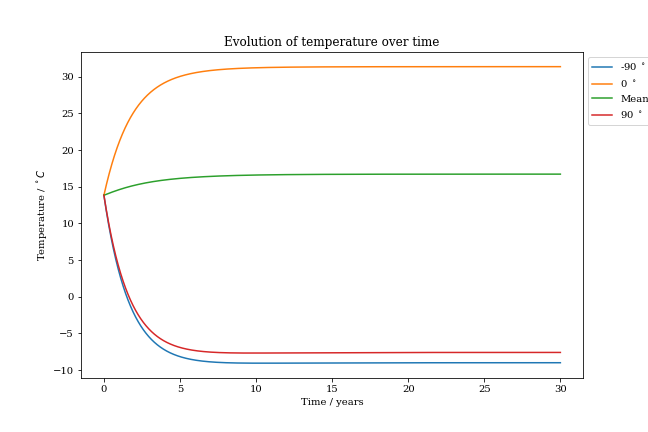
\includegraphics[width=225px]{temperature-evolution.png}%
    \caption{Evolution of temperature over time}%
  \end{subfigure}
  \caption{Graphical results from the inital python simulation}
\end{figure}

Figure 1 (a) gives a good insight into the overall behaviour of the forward difference equation as it progresses through the timesteps.
The line at T = 13.85$^\circ C$ represents the initial setting of the global temperature in the programme.
It shows that as time progresses the curve becomes narrower and peaks towards the $0 ^\circ $ latitidue. 
The simulation also shows diminishing returns in terms of temperature increase as time progresses and the system approaches equilibrium.
I thought that it would be interesting to see how the simulation progressed visually. I have created a short animated version of Figure 1 (a) which is available at this link. [\url{https://github.com/Birr0/physics_labs/blob/main/climate_modelling/climate.gif}]

\begin{figure}[H]%
  \centering%
  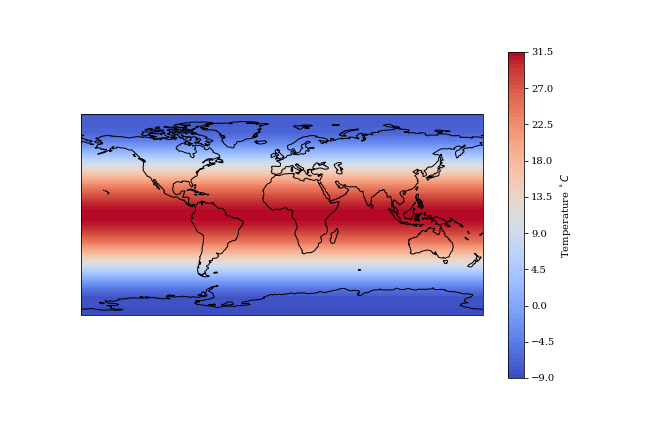
\includegraphics[width=350px]{global-temp-distribution.png}
  \caption{Contour plot of temperature distribution from the 1D EBM simulation after 30 years}
\end{figure}

Figure 2 is a more initutive respresentation of Figure 1 (a). You can see the gradation in temperature from the dark red at the equator to the deep blues at the poles.
Figure 2 also is subtle in pointing out the difference in shades of blue between the poles as demonstrated in figure 1 (a). The south pole is slightly cooler than the north pole. 
Our polynomial equation modelling the albedo as a function of latitude has a larger albedo value at the south pole compared to the north. \cite{Lacis}
This is to reflect the higher albedo at the south pole due to the year round snow and excess ice at the south pole. \par
However, there is disagreement between the model with the experimental data. From Feulner et. al \cite{Feulner} there is significant deviation from the CRU dataset (1961-90) at both poles, especially the south pole.
Factors not included in our model such as the influence of land and ice-sheet elevation results in vastly lower temperatures in Antartica. \cite{Feulner} 

\subsection{Modelling the effect of the infared transmission paramter, $ \tau$ }
The transmission parameter $\tau$, describes the fraction of infrared light that is emitted by the earth's atmosphere. It is dictated mainly by the concentration of greenhouse
gases in the atmosphere. Therefore, changing this parameter in our simulation represents changing the composition of the atmosphere. \par
The emission of infrared light has a cooling effect on the earth. One would expect then that a greater transmission coefficient would lead to cooler temperatures.
An initial plot of the equatorial temperature distribution helps to confirm this hypothesis.

\begin{figure}[H]%
  \centering%
  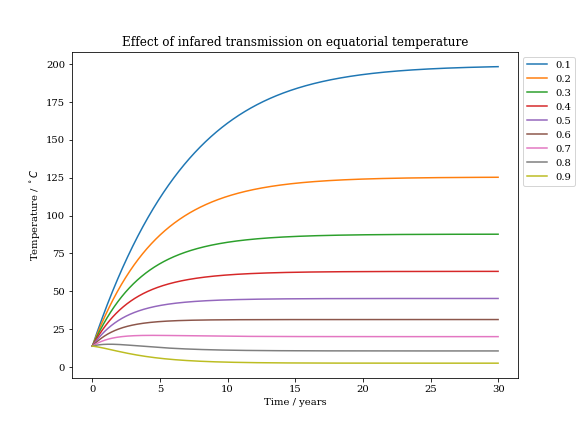
\includegraphics[width=250px]{temperature-distributions-IR.png}
  \caption{Equatorial temperature distribution plots for $ 0 < \tau < 1$}
\end{figure}

Figure 3 shows with that with a lower percentage transmission of infrared, the equilibrium temperature of the equator increases significantly. 
What is the nature of the relationship between temperature and $\tau$ ? 

\begin{figure}[H]%
  \centering%
  \begin{subfigure}{0.4\textwidth}
    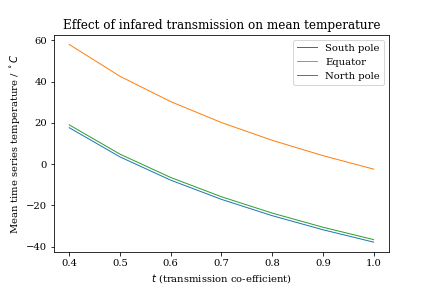
\includegraphics[width=225px]{mean-temperature-IR.png}
    \caption{Mean temperature plots for $ 0.4 \le \tau < 1 $}
  \end{subfigure}
  \begin{subfigure}{0.4\textwidth}
    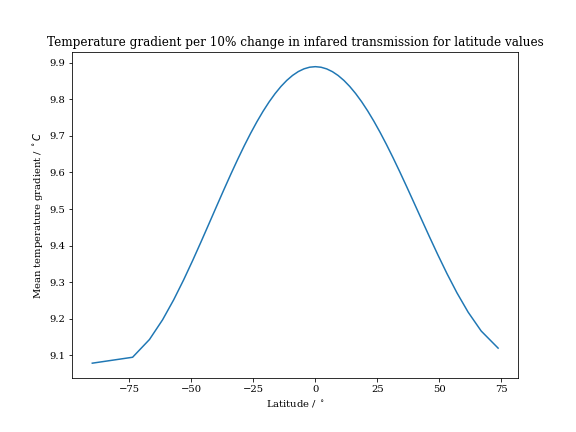
\includegraphics[width=225px]{Temperature-grad-tau.png}
    \caption{Temperature gradient for every 10$ \%$ increase in $ \tau$}
  \end{subfigure}
  \caption{Modelling the effect of $\tau$ on our python simulation}
\end{figure}

Between $ 0.4 \le \tau < 1 $, the relationship between temperature and $\tau$ could be approximated to be linear within these bounds.

By applying a linear regression model across the temperature distribution at t = 30 years, I estimate that for every 10 \% decrease in IR transmission 
there is a resultant 9.59 $^\circ C$ increase in temperature ($ R^2 = 0.977$). We also see from figure 4 (b) that this effect is more pronuced at the poles. 
However, observation in the literature indicates that the poles are warming at a faster rate than the equator. 
The consensus is that rising temperatures in the polar regions cause the polar icecaps to melt. This has the effect of lowering the albedo term in equation 1)
and creates a 'positive' feedback mechanism to increase the temperature of the polar regions further and decrease the albedo. \cite{NASA}
 This reflects a serious limitatiton in my model, were the albedo feedback mechanism is ignored.

\subsection{The thermal conductivity of Earth}
In our simulation another important parameter to consider is the thermal conductivity, k. 
In our simulation it governs the earth's ability to conduct heat across latitudes.
Figure 5) demonstrates how various values of k influence the temperature distribution for latitude = $0^\circ$.

\begin{figure}[H]%
    \centering
    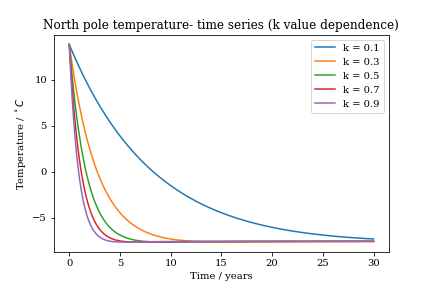
\includegraphics[width=300px]{north-pole-k-variation.png}
    \caption{Various temperature distributions with K variations for latitude = $90 ^\circ $}
\end{figure}

What is evident from figure 5) is that K has a non-significant effect on equilbrium temperature but is very influential in 
determining the rate at which equilibrium is reached. For higher values of K, equilibrium temperature is reached much more quickly.

\subsection{Estimating the time taken for 1D FDM to reach thermal equilibrium}
We can get a crude estimate for the time taken for earth to reach thermal equilbrium by an analytical solution of the 0D energy balance equation, given by \cite{Rose}

\begin{equation}
  C \frac{dT_{s}}{dt} = (1 - \alpha)Q - \sigma(\beta T_{s})^4 
\end{equation}
Where C is the specific heat capacity of the earth, $T_{s}$ is the surface temperature ,$ (1 - \alpha)Q $ is the heat input after accounting for albedo, $\alpha$ and $\sigma(\beta T_{s})^4$ is the heat output.
We can begin the process of linearizing this equation. 
The equilbrium surface temperature, $ \overline{T_{s}}$ can be written as

\begin{equation}
  \overline{T_{s}} = \frac{1}{\beta}(\frac{1 - \alpha}{\sigma})^{\frac{1}{4}} = 287K
\end{equation}
If we let the surface temperature be the equilbrium be

$$ T_{s} = \overline{T_{s}} + {T'_{s}} $$ where ${T'_{s}}$ is a small perturbation in the temperature bound by ${T'_{s}} << \overline{T_{s}}$.

Next, we can use a first order Taylor expansion to to write the heat emitted by the earth as

$$\sigma(\beta T_{s})^{4} \approx \sigma(\beta \overline{T_{s}})^{4} + (4\sigma \beta^4 \overline{T_{s}}^3){T'_{s}} $$
From equation (10) $$ (1 - \alpha)Q = \sigma( \beta \overline{T_{s}})^4 $$

equation (9) becomes 

$$C \frac{dT'_{s}}{dt} = (1 - \alpha)Q - ( (1 - \alpha)Q +(4\sigma \beta^4 \overline{T_{s}}^3){T'_{s}}) $$

Therfore,
\begin{equation}
  \frac{dT'_{s}}{dt} = \frac{{T'_{s}}}{\tau}
\end{equation}

where $$ \tau = -\frac{C}{4\sigma \beta^4 \overline{T_{s}}^3} $$.

We can solve this linearized first order differential equation as follows:
$$ \int_{{T'_{s}}(0)}^{{T'_{s}}(t)} \frac{d {T'_{s}}}{T_{s}} = \int_{0}^{t} \frac{dt}{\tau}$$

\begin{equation}
  {T'_{s}}(t) = {T'_{s}}(0) exp(-\frac{t}{\tau})
\end{equation}

The significance of $\tau$ is revealed here as the e-folding time, i.e. the time taken for the temperature pertubation to decay to $\frac{1}{e}$ of the intial pertutbation.
This acts as a good approximation for the time taken to reach equilbrium for the 0D case. 

Estimating the specific heat capacity of the earth to be 3.5 $\cdot 10^{8} JK^{-1}m^{-2}$ we can estimate the time taken to reach equilbrium to be 
$ \tau = 3.36 $ years.

From my analysis, the change in global mean temperature falls by $\frac{1}{e}$ of it's initial pertubation after 5.56 years for K=0.6. This difference of two years is prehaps due to differences between the models.
For example, I have incorporated the thermal conductivity of the earth into the python simulation which plays a significant role in determining when equilbrium is reached. When the calculation is altered to use K = 1.0, I get an estimate much closer at 2.78 years.

\section{Conclusion}
I have derived the finite difference model from the one dimensional energy balance equation and implemented a python program to simulate 
the finite difference model over a 30 year period. I have explored the impact of the $\tau$ and K parameters on the simulation and estimated the time required for 
the system to reach equilibrium. I have also discussed the limitations of the model with respect to experimental results. Further analysis with regards to albedo feedback mechanism would be useful in order to generate a much more 
realistic model.
%
\printbibliography
%
\end{document}